\documentclass[a4paper,10pt]{article}

% рисунки
\usepackage{graphicx}

\usepackage[T2A]{fontenc}
\usepackage[utf8]{inputenc}
\usepackage[english,russian]{babel}

\RequirePackage{caption}
\DeclareCaptionLabelSeparator{defffis}{ — }
\captionsetup{justification=centering,labelsep=defffis}

\usepackage{caption} \captionsetup[table]{labelsep=endash,justification=justified,singlelinecheck=false,font=normalsize}

\usepackage{amsmath,amsfonts,amssymb,amsthm,mathtools}



\begin{document}
  
\begin{center}
  \section*{Лабораторная работа №3.2.4 \\Свободные колебания в электрическом контуре\\Джокер Бэтмен, Б02-000, 25.09.2021}
\end{center}  

\vspace{5mm}
\section*{Введение}

\begin{flushleft}
  \textbf{Цель работы:} исследование свободных колебаний в электрическом колебательном контуре.

\end{flushleft}

\begin{flushleft}
  \textbf{В работе используются:} генератор импульсов, электронное реле, магазин сопротивлений, магазин ёмкостей, катушка индуктивности, электронный осциллограф с разделительной панелью, измеритель $RLC$.

\end{flushleft}

\section*{Теоретическая справка}

Условие реализации режима затухающих колебаний в $LCR$-контуре имеет вид\[0 < R < 2\sqrt{\frac{L}{C}}=R_{\text{кр}},\]где $R_{\text{кр}}$ -- \textit{критическое сопротивление}.

При выполнении этого условия напряжение $U_C(t)$ на конденсаторе зависит от времени как\[U_C(t)=U_0e^{-\gamma t}\cos{\left(\omega_1t+\varphi_0\right)}.\]Здесь $\gamma=\frac{R}{2L}$, а $\omega_1=\sqrt{\frac{1}{LC}-\frac{R^2}{4L^4}}$.

Несложно заметить, что выражения для напряжения $U_C(t)$ и тока $I(t)$ можно при должном подборе начальной фазы записать в виде
\begin{flalign*}
&U_C(t)=U_{C0}e^{-\gamma t}\left(\cos{\omega_1t}+\frac{\gamma}{\omega_1}\sin{\omega_1t}\right),&&\\
&I(t)=C\dot{U}_C=-\frac{2U_{C0}}{R_{\text{кр}}}\frac{\omega_0}{\omega_1}e^{-\gamma t}\sin{\omega_1t}.&&
\end{flalign*}

С помощью этих формул можно параметрически представить \textit{траектории системы на фазовой плоскости} переменных $(U_C,I)$.

На рисунке \Ref{th}, а) показаны зависимости напряжения и тока в контуре от времени \textit{в безразмерных переменных} $u(x)=\frac{U_C(x)}{U_{C0}},\ j(x)=\frac{R_{\text{кр}}I(x)}{2U_{C0}},\ \text{где}\ x=\frac{\omega_1t}{2\pi}$. На рисунке \Ref{th}, б) показана фазовая траектория этих колебаний на плоскости $(u,j)$, представляющая собой скручивающуюся к точке $(0,0)$ спираль.

\begin{figure}[h]
	\centering
	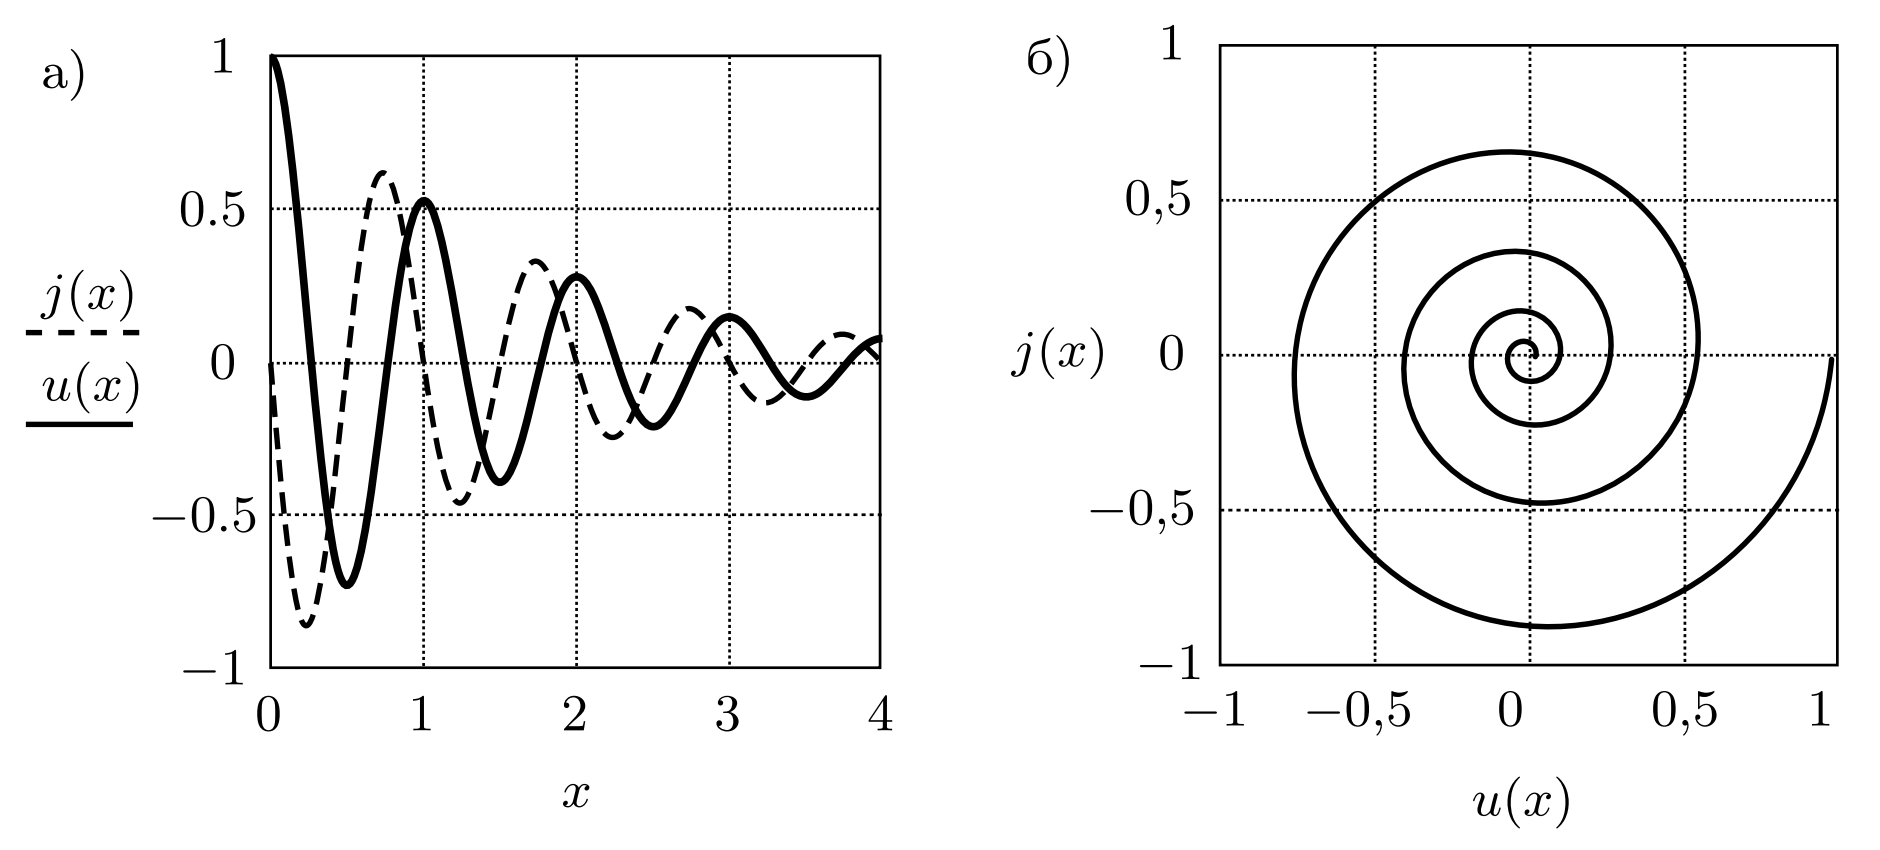
\includegraphics[scale=0.24]{th}
	\caption{Затухающие колебания: а) ток в контуре $j(x)$ и напряжение на конденсаторе $u(x)$, б) траектория системы на фазовой плоскости $(u,j)$} \label{th}
\end{figure}

\textit{Период затухающих колебаний} равен\[T_1=\frac{2\pi}{\omega_1} > T_0,\]т.е. наличие потерь в контуре приводит к увеличению периода колебаний.

Другими характеристиками процесса затухания являются \textit{время затухания}\[\tau=\frac{2L}{R},\] за которое амплитуда колебаний убывает в $e$ раз, и \textit{логарифмический декремент затухания}\[\Theta=\ln{\frac{U_k}{U_{k+1}}}=\gamma T_1,\]где $U_k$ и $U_{k+1}$ -- два последовательных максимума рассматрваемой величины.

С логарифмическим декрементом связана ещё одна важнейшая характеристика колебательного контура -- его \textit{добротность} $Q$:\[Q\equiv\frac{\pi}{\Theta}=\frac{1}{2}\sqrt{\frac{R_{\text{кр}}^2}{R^2}-1}.\]

При $Q\gg1$ можно с хорошей точностью заменить $\omega_1$ на $\omega_0$ в уравнениях для зависимости напряжения и тока в контуре от времени, что вносит относительную погрешность порядка $\frac{1}{Q^2}$.

\section*{Экспериментальная установка}

На рисунке \Ref{Device} приведена схема установки для исследования свободных колебаний в контуре, содержащем постоянную индуктивность $L$ с активным сопротивлением $R_L$, а также переменные ёмкость $C$ и сопротивление $R$. Картина колебаний напряжения на ёмкости наблюдается на экране двухканального осциллографа. Выходные клеммы ЭО выведены на отдельную панель П.

Для периодического возбуждения колебаний в контуре используется генератор импульсов Г5-54. С выхода генератора по коаксиальному кабелю импульсы поступают на колебательный контур через электронное реле, смонтированное в отдельном блоке. Реле содержит диодный тиристор $D$ и ограничительный резистор $R_1$.

\begin{figure}[h]
	\centering
	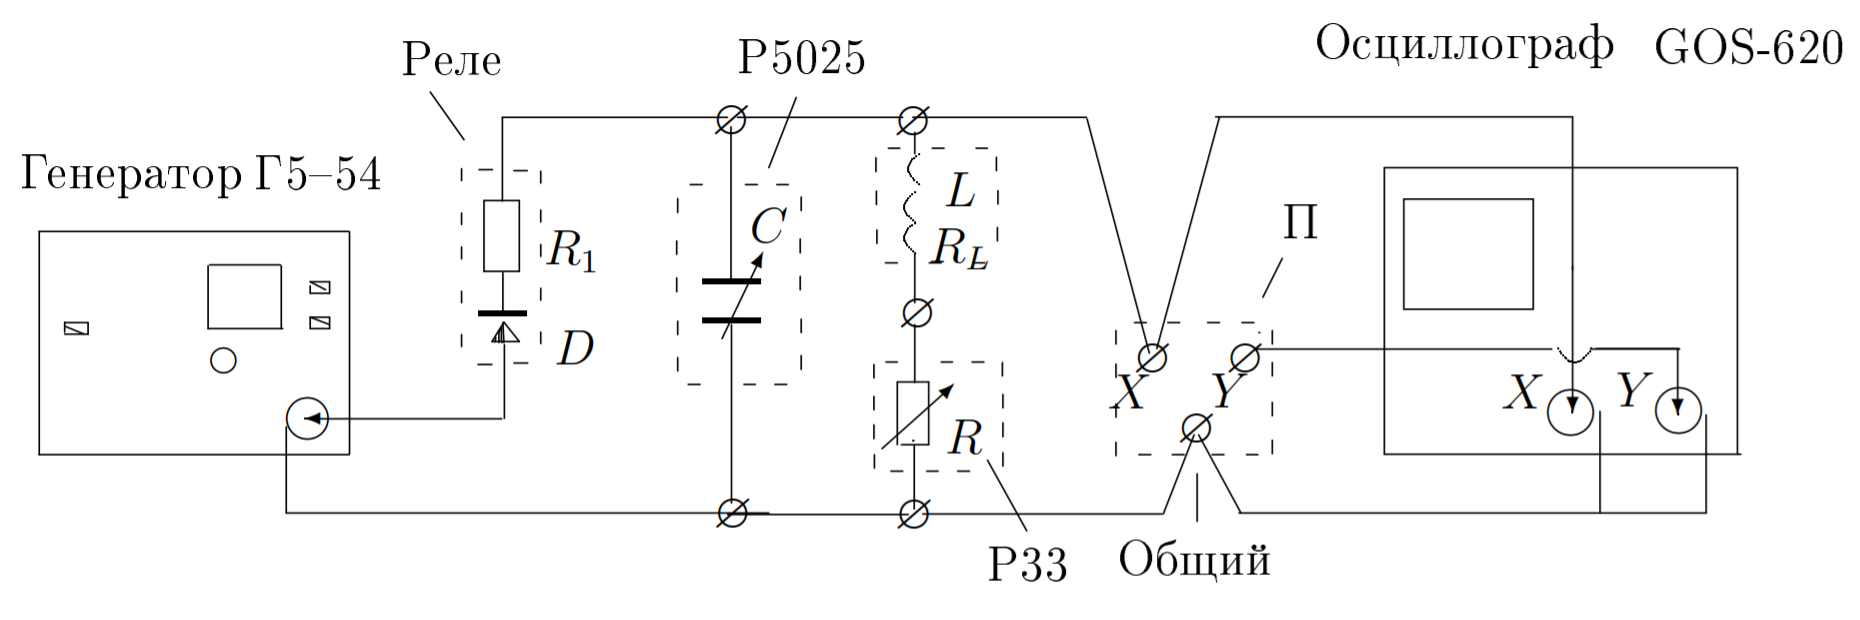
\includegraphics[scale=0.25]{Device}
	\caption{Схема установки для исследования свободных колебаний} \label{Device}
\end{figure}

Каждый импульс заряжает конденсатор $C$, после чего генератор отключается от колебательного контура, и в контуре возникают свободные затухающие колебания. Напряжение на конденсаторе $U_C$ поступает на вход канала $X$ ЭО, а напряжение на сопротивлении $R$, пропорциональное току $I$ в контуре ($I\propto\frac{\text{d}U_C}{\text{d}t}$), поступает на вход канала $Y$. В двухканальном режиме работы ЭО а экране можно наблюдать затухающие колебания напряжения и тока одновременно, а при отключении внутренней развёртки ЭО -- в режиме $X-Y$ -- фазовую диаграмму. Входное сопротивление осциллографа велико ($\approx1~\text{М}\Omega$), так что его влиянием на контур можно пренебречь.

При включенной развёртке по времени картина затухающих колебаний представлена в координатах $(t,U_C)$ и $(t,\frac{\text{d}U_C}{\text{d}t})$, при выключенной -- в координатах $(U_C,\frac{\text{d}U_C}{\text{d}t})$. В этих координатах картина незатухающих коебаний (при $\gamma=0$) представляет собой эллипс, а затухающих (при $\gamma > 0$) -- скручивающуюся спираль.

\section*{Ход работы}

Перед началом работы подключим генератор через реле ко входу $X$ ЭО и запустим на генераторе прямоугольные импульсы частотой $\nu_0=100~\text{Гц}$, длительностью $\sim5~\text{мкс}$ и амплитудой $\approx30~\text{В}$. Настроив осциллограф, проверим, совпадает ли период повторения импульсов, указанный на генераторе, с измерениями по горизонтальной шкале ЭО. Видим, что при развёртке $1~\text{мс}$ период импульса занимает на экране $9,9$ делений т.е. отклонение составляет примерно $1\%$ при указанном в ТО осциллографа максимальном отклонении $3\%$, что позволяет сделать вывод о работоспособности ЭО.

Подберём развёртку так, чтобы на экране умещалось несколько импульсов. Зарегистрированная при этом картина качественно показана ниже на рисунке \Ref{fig}.

\begin{figure}[h]
	\centering
	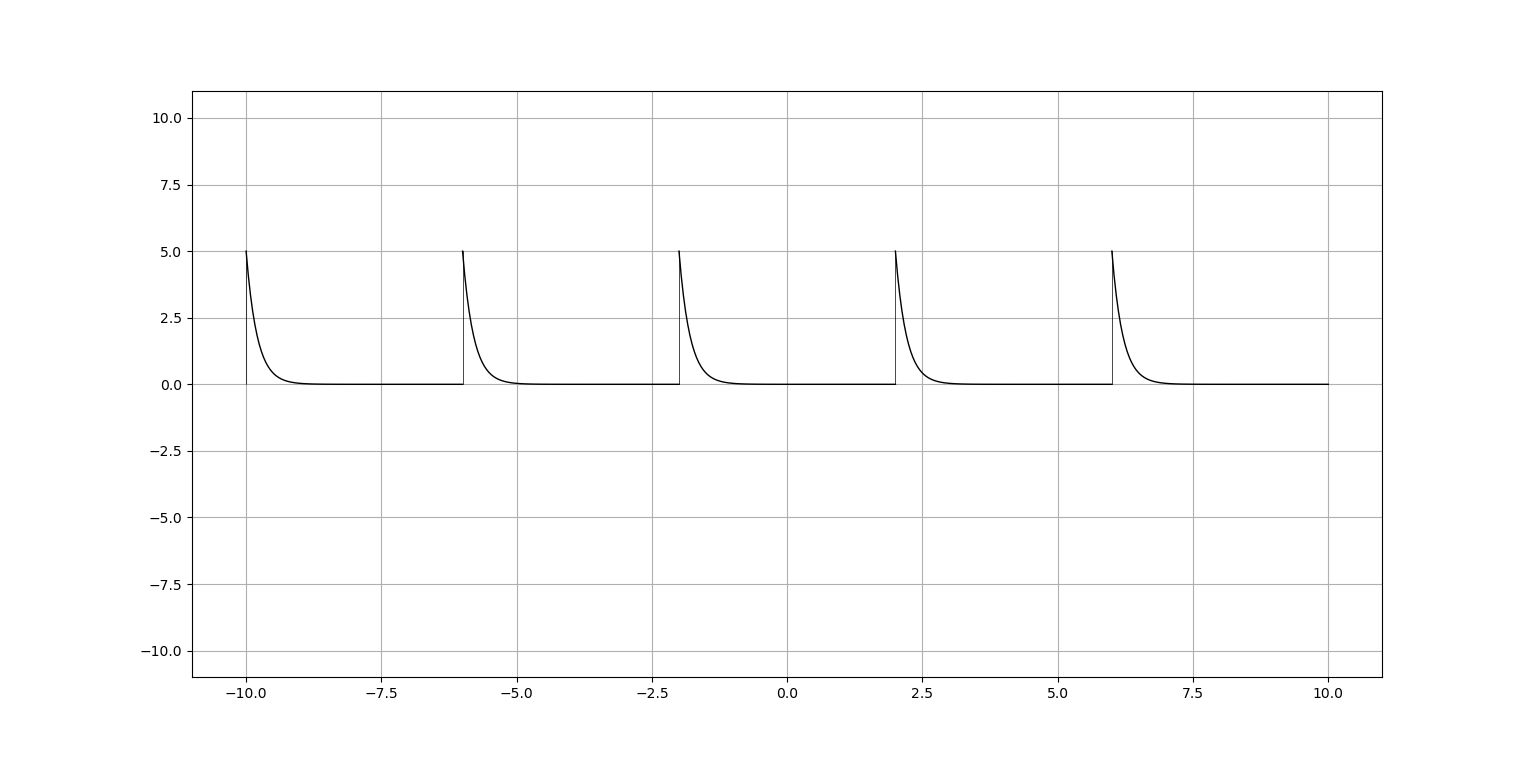
\includegraphics[scale=0.33]{fig}
	\caption{Регистирируемая при подготовке приборов к работе картина на экране осциллографа} \label{fig}
\end{figure}

\subsection*{I. Измерение периодов свободных колебаний}

Соберём схему согласно рисунку \Ref{Device}. Установим на магазине сопротивлнеий величину $R=0$, а на магазине ёмкостей -- величину $C=0,02~\text{мкФ}$. Получим на экране ОЭ картину свободных затухающих колебаний, подобрав частоту развёртки так, чтобы расстояние $x_0$ между импульсами, поступающими с генератора, занимало почти весь экран. В настоящей работе оно равно $9,8\pm0,1$ дел.

Измерим на экране расстояние $x$, которое занимают несколько полных периодов $n$. Зная период задающих колебания импульсов $T_0=\frac{1}{\nu}=0,01~\text{с}$ и $x_0$, найдём период колебаний контура:\[T=\frac{T_0x}{nx_0}.\]Для оценки погрешностей заметим, что относительная погрешность определения длины нескольких периодов сравнима с относительной погрешностью определения $x_0$, тогда относительная погрешность определения периода затухающих колебаний складывается из удвоенного вклада погрешности определения $x_0$ и погрешности определения $T_0$, откуда $\varepsilon_T=1,5\%$.

Проведём измерения периодов при постоянном $x_0$, изменяя ёмкость в диапазоне от 0,02 мкФ до 0,90 мкФ. Занесём полученные данные в талицу \Ref{per}. Занесём в таблицу также значения периода, рассчитанные по теоретической формуле $T=2\pi\sqrt{LC}$. Будем использовать значение $L=\left(199,22\pm0,20\right)~\text{мГн}$, измерение которого будет описано в части III Хода работы.

\begin{table}[h]
	\centering
	\caption{Зависимость периода $T$ затухающих колебаний от ёмкости $C$} \label{per}
	\begin{tabular}{|c|c|c|c|c|c|c|c|c|c|c|}
		\hline
		$C$,мкФ&0,02&0,05&0,10&0,20&0,30&0,40&0,50&0,60&0,75&0,90\\ \hline
		$x$,делВ&9,5&9,4&8,8&8,7&7,7&8,8&7,9&8,7&7,3&8,0\\ \hline
		$n$&24&15&10&7&5&5&4&4&3&3\\ \hline
		$T$,мс&0,40&0,63&0,88&1,24&1,54&1,76&1,98&2,18&2,43&2,67\\ \hline
		$T_{th}$,мс&0,40&0,63&0,89&1,25&1,54&1,77&1,98&2,17&2,43&2,66\\ \hline
	\end{tabular}
\end{table}

Видим, что значения $T$ и $T_{th}$ очень точно совпадают в пределах погрешностей, что говорит о точности исходных измерений. Относительная погрешность определения периода равна половине относительной погрешности определения $L$, равной $0,1\%$. Зная всё это, построим для наглядности график $T(T_{th})$, который представлен ниже на рисунке \Ref{rofl}.

\begin{figure}[h]
	\centering
	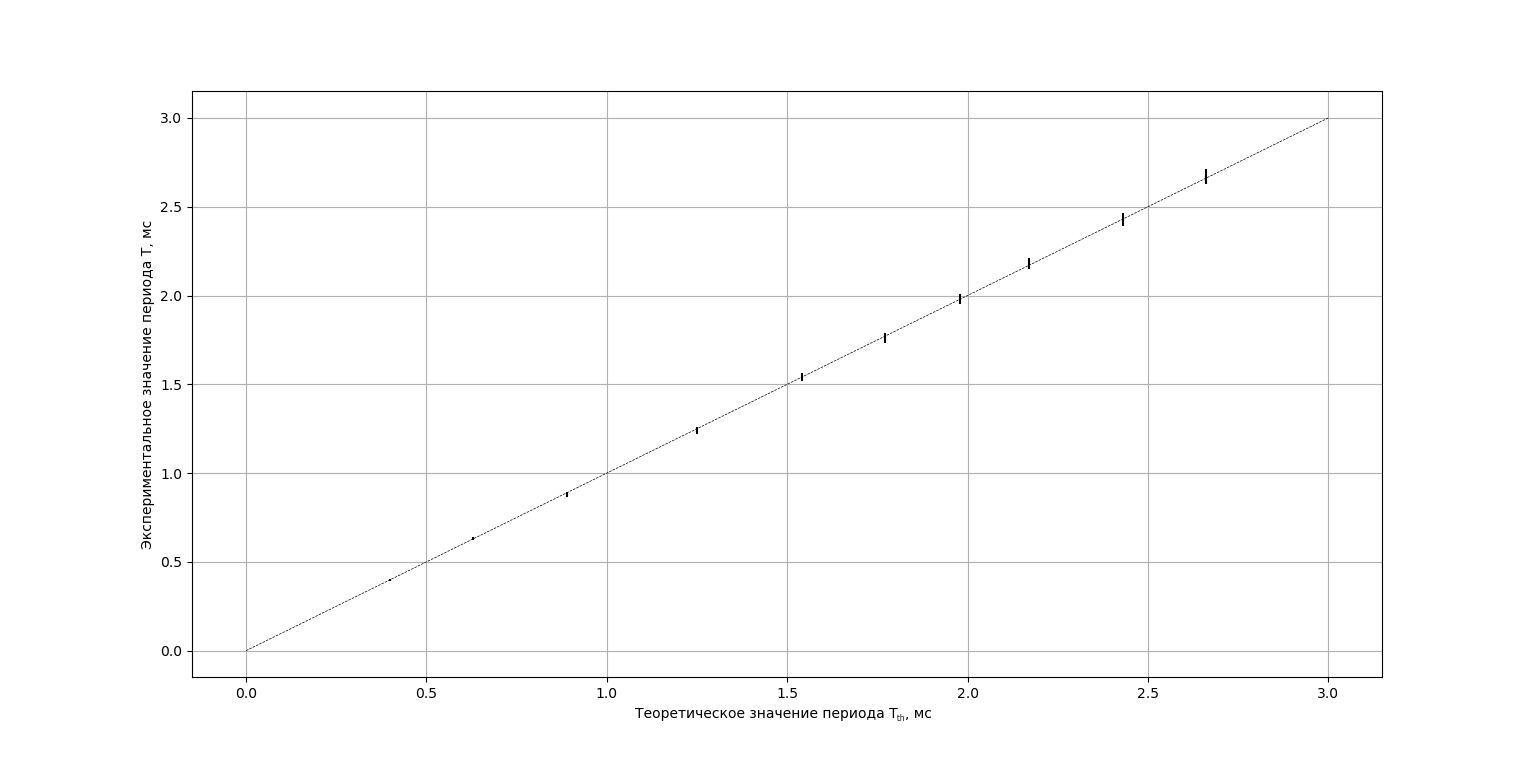
\includegraphics[scale=0.33]{rofl}
	\caption{Зависимость экспериментального значения периода затухающих колебаний $T$ от теоретического $T_{th}$. Прямая проведена с помощью МНК} \label{rofl}
\end{figure}

\subsection*{II. Критическое сопротивление и декремент затухания}

Приняв $L=200~\text{мГн}$, рассчитаем ёмкость $C$, при которой собственная частота колебаний контура $\nu_0=\frac{1}{2\pi\sqrt{LC}}$ составит 5 кГц. Получим значение $C=\frac{1}{4\pi^2\nu_0^2L}=0,00507~\text{мкФ}$. Рассчитаем также критическое сопротивление контура с такими параметрами, оно равно $R_{\text{кр}}=4\pi\nu_0L=12566~\Omega$.

Установим на магазине ёмкость $C=0,005~\text{мкФ}$, наиболее близкую к рассчитанной выше. Будем увеличивать сопротивление $R$ от нуля до $R_{\text{кр}}$, наблюдая картину затухающих колебаний на экране ЭО. Колебательный режим переходит в апериодический примерно при $R_{\text{кр}}=12000~\Omega$, будем в дальнейшем использовать его.

Приступим к измерению логарифмического декремента затухания. Установим сопротивление $R=0,1R_{\text{кр}}=1200~\Omega$. Получим на экране ЭО картину колебаний. Сместим горизонтальную ось симметрии вниз экрана для повышения точности измерений. Несложно показать, что при декременте $\Theta\geq\ln2$ абсолютная погрешность измереия будет лишь расти с увеличением числа разделяющих максимумы периодов, поэтому для почти всех $R$ будем измерять лишь отношение соседних максимумов. Проведём измерения для 8 различных значений $R$ в диапазоне от $0,1R_{\text{кр}}$ до $0,3R_{\text{кр}}=3600~\Omega$. Логарифмический декремент затухания находится по формуле\[\Theta=\frac{1}{n}\ln{\frac{A_k}{A_{k+n}}}.\]Абсолютная погрешность $\sigma_{\Theta}$ получается из относительных погрешностей измерения амплитуд $A_i$ и $A_f$ (погрешность величин, выбираемых на магазинах, считаем пренебрежимо малой). Занесём все результаты в таблицу \Ref{decr}.

\begin{table}[h]
	\centering
	\caption{Зависимость логарифмического декремента затухания $\Theta$ от сопротивления контура $R$} \label{decr}
	\begin{tabular}{|c|c|c|c|c|c|c|c|c|}
		\hline
		$\frac{R}{R_{\text{кр}}}$ & 0,100 & 0,125 & 0,150 & 0,175 & 0,200 & 0,225 & 0,250 & 0,300 \\ \hline
		$R,\ \text{к}\Omega$ & 1,2 & 1,5 & 1,8 & 2,1 & 2,4 & 2,7 & 3,0 & 3,6 \\ \hline
		$A_i$, дел & 7,4 & 7,4 & 7,4 & 7,4 & 7,4 & 7,4 & 7,4 & 7,4 \\ \hline
		$A_f$, дел & 1,0 & 3,4 & 2,8 & 2,4 & 2,0 & 1,7 & 1,4 & 1,0 \\ \hline
		$n$ & 3 & 1 & 1 & 1 & 1 & 1 & 1 & 1 \\ \hline
		$\Theta$ & 0,67 & 0,78 & 0,98 & 1,13 & 1,31 & 1,47 & 1,67 & 2,00 \\ \hline
		$\sigma_{\Theta}$ & 0,03 & 0,03 & 0,04 & 0,04 & 0,05 & 0,06 & 0,07 & 0,10 \\ \hline
		$X,\ 10^{-7}\Omega^{-2}$ & 6,52 & 4,23 & 2,96 & 2,19 & 1,68 & 1,33 & 1,08 & 0,76 \\ \hline
		$Y$ & 2,23 & 1,64 & 1,04 & 0,78 & 0,58 & 0,46 & 0,36 & 0,25 \\ \hline
		$\sigma_Y$ & 0,20 & 0,13 & 0,08 & 0,06 & 0,04 & 0,04 & 0,03 & 0,03 \\ \hline
	\end{tabular}
\end{table}

В дальнейшем в работе будет измерено омическое сопротивление витков катушки при 5 кГц, которое равно $R_L=\left(38,40\pm0,04\right)~\Omega$. Видим, что тогда при вычислении $R_{\Sigma}=R+R_L$ погрешностью $\sigma_{R_L}$ можно будет пренебречь (в особенности по сравнению с погрешностью определения декремента).

Приняв обозначения $X=\frac{1}{R_{\Sigma}^2}$ и $Y=\frac{1}{\Theta^2}$, можно показать, что $R_{\text{кр}}=2\pi\sqrt{\frac{\Delta Y}{\Delta X}}$. Вычислим величины $X$, $Y$ и $\sigma_Y$ и тоже занесём их в таблицу \Ref{decr}.

Построим график $Y(X)$. Он представлен ниже на рисунке \Ref{ddecr}. Помимо того, что для определения критического сопротивления можно использовать наклон графика, ясно, что точка пересечения графика с осью $X$ соответствует точке, в которой логарифмический декремент затухания устремляется к бесконечности, т.е. к точке перехода к апериодическому режиму, а значит, $X$-координата этой точки равна $R_{\text{кр}}^{-2}$.

\begin{figure}[h]
	\centering
	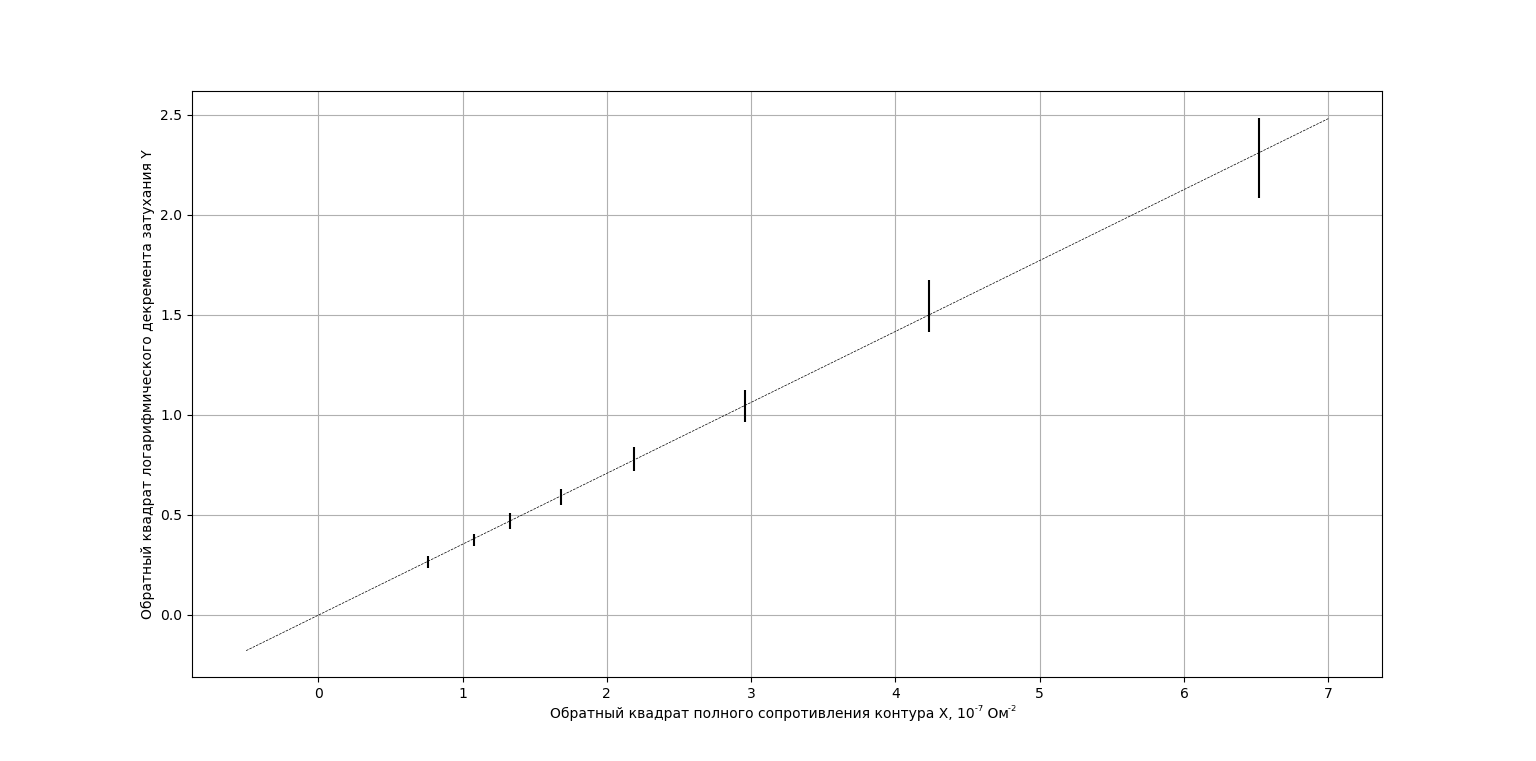
\includegraphics[scale=0.33]{ddecr}
	\caption{График в координатах $X-Y$ для определения критического сопротивления. Прямая проведена с помощью МНК} \label{ddecr}
\end{figure}

Непосредственно из графика находим $\frac{\Delta Y}{\Delta X}=\left(3,65\pm0,32\right)\cdot10^6~\Omega^2$, откуда находим $R_{\text{кр}}=\left(12,34\pm0,53\right)~\text{к}\Omega$. Видим, что при этом определить критическое сопротивление по точке пересечения графика с осью абсцисс в какой бы то ни было вменяемой точностью практически невозможно.

Теоретическое значение критического сопротивления $R_{\text{кр}}=2\sqrt{\frac{L}{C}}=\left(12,624\pm0,006\right)~\text{к}\Omega$, т.е. в пределах погрешности оно совпадает с полученным в эксперименте.

\subsection*{III. Свободные колебания на фазовой плоскости}

Переключим ЭО на двухканальный режим для одновременного наблюдения осциллограмм тока и напряжения. Подберём масштабы и частоту развёртки так, чтобы оба сигнала были представлены на временном интервале, слегка превышающем период повторения импульсов с генератора. Полученная картина будет качественно совпадать с показанной на рисунке \Ref{th}, а).

Для наблюдения затухающих колебаний на фазовой плоскости переключим развёртку ЭО в положение $X-Y$. На магазине сопротивлений выберем значение $R=0,1R_{\text{кр}}$. Подберём масштаб спирали, удобный для измерений. Спираль качественно совпадает с теоретической, показанной на рисунке \Ref{th}, б). Для повышения точности при измерениях будем сдвигать центр спирали к краям экрана.

При том же значении $C$, что и в части II Хода работы, пронаблюдаем за изменением спирали при увеличении сопротивления от 0,1 до 0,3$R_{\text{кр}}$. Видим, что спираль закручивается слабее и становится менее плотной с ростом $R$.

Для определения $\Theta$ измерим максимумы $A_i$ и $A_f$ отклонения витков спирали по оси $x$, разделёных целым число периодов $n$, для максимального и минимального значений $R$ из использованного в работе диапазона. Занесём результаты в таблицу \Ref{lst}. Погрешность $\Theta$ здесь будет определяться аналогично. Также внесём в таблицу значения добротности контура, рассчитанное теретически из величин его параметров, а также значения добротности, вычисленные по формуле\[Q=\frac{\pi}{\Theta},\]и величину погрешности $\sigma_Q$.

\begin{table}[h]
	\centering
	\caption{Зависимость добротности контура $Q$ от сопротивления $R$, измеренная с помощью спирали на фазовой плоскости} \label{lst}
	\begin{tabular}{|c|c|c|c|c|c|c|c|}
		\hline
		$\frac{R}{R_{\text{кр}}}$ & $A_i$ & $A_f$ & $n$ & $\Theta$ & $Q_{th}$ & $Q$ & $\sigma_Q$ \\ \hline
		0,1 & 7,4 & 1,1 & 3 & 0,64 & 5,26 & 5,02 & 0,24 \\ \hline
		0,3 & 7,4 & 1,1 & 1 & 1,91 & 1,73 & 1,68 & 0,08 \\ \hline
	\end{tabular}
\end{table}

Наконец, отсоединим катушку от цепи и измерим её омическое сопротивление $R_L$ и индуктивность $L$ с помощью измерителя $LCR$ при значениях частоты 50 Гц, 1 кГц и 5 кГц. Занесём результаты измерений в таблицу \Ref{zaeblo}. Отметим, что погрешность измерения измерителя $LCR$ равна $0,1\%$.

\begin{table}[h]
	\centering
	\caption{Внутреннее сопротивление катушки $R_L$ и её индуктивность $L$ при различных частотах $\nu$ переменного тока} \label{zaeblo}
	\begin{tabular}{|c|c|c|c|}
		\hline
		$\nu$, кГц & 0,05 & 1,00 & 5,00 \\ \hline
		$R_L,\ \Omega$ & 11,04 & 18,62 & 38,40 \\ \hline
		$L$, мГн & 203,8 & 199,2 & 199,2 \\ \hline
	\end{tabular}
\end{table}

Стоит отметить, что результат измерения $R$ зависит от частоты. Это происходит потому, что вклад в активное сопротивление катушки вносят омические потери не только в витках катушки, но и в её сердечнике, а также потери на перемагничивание, очевидно растущие с увеличением частоты.

\section*{Вывод}

В данной работе были исследованы свободные колебания в электрическом колебательном контуре.

В первой части работы был измерен период свободных затухающих колебаний, и экспериментально с высокой точностью была подтверждена соответствующая теоретическая зависимость.

Во второй части работы был измерен декремент затухания контура. С его помощью было найдено критическое сопротивление контура $R_{\text{кр}}=\left(12,34\pm0,53\right)~\text{к}\Omega$, в пределах погрешности совпадающее с теоретически предсказанным $R_{\text{кр}}=\left(12,624\pm0,006\right)~\text{к}\Omega$, что говорит о точности используемого метода.

В третьей части работы были исследованы свободные колебания на фазовой плоскости, зарегистрирована спираль и её поведение при изменении сопротивления контура. Была измерена добротность контура $Q$, полученные значения при различных сопротивлениях (см. таблицу \Ref{lst}) в пределах погрешностей совпали с теоретически предсказанными, что вновь говорит о точности и корректности проведённых измерений.

\end{document}
